
\documentclass [11pt]{report}

\usepackage{fancyhdr}
\usepackage [french]{babel}

\usepackage[utf8]{inputenc}
\usepackage[T1]{fontenc}
\usepackage{textcomp}
\usepackage{graphicx}
\usepackage[a4paper]{geometry}
\usepackage{titlepic}
\usepackage{boxedminipage}
\usepackage{listings}
\usepackage{minitoc}
\usepackage{footmisc}
\usepackage{color}
\usepackage{graphicx}
\usepackage{fancyvrb}

\usepackage{eso-pic}

\makeatletter
\newlength\@tempdim@x
\newlength\@tempdim@y
% structure des commandes :
%   #1 = deplacement selon x
%   #2 = deplacement selon y
%   #3 = texte à mettre
\newcommand\AtUpperLeftCorner[3]{%
\begingroup
\@tempdim@x=0cm
\@tempdim@y=\paperheight
\advance\@tempdim@x#1
\advance\@tempdim@y-#2
\put(\LenToUnit{\@tempdim@x},\LenToUnit{\@tempdim@y}){#3}%
\endgroup
}
\newcommand\AtUpperRightCorner[3]{%
\begingroup
\@tempdim@x=\paperwidth
\@tempdim@y=\paperheight
\advance\@tempdim@x-#1
\advance\@tempdim@y-#2
\put(\LenToUnit{\@tempdim@x},\LenToUnit{\@tempdim@y}){#3}%
\endgroup
}
\newcommand\AtLowerLeftCorner[3]{%
\begingroup
\@tempdim@x=0cm
\@tempdim@y=0cm
\advance\@tempdim@x#1
\advance\@tempdim@y#2
\put(\LenToUnit{\@tempdim@x},\LenToUnit{\@tempdim@y}){#3}%
\endgroup
}
\newcommand\AtLowerRightCorner[3]{%
\begingroup
\@tempdim@x=\paperwidth
\@tempdim@y=0cm
\advance\@tempdim@x-#1
\advance\@tempdim@y#2
\put(\LenToUnit{\@tempdim@x},\LenToUnit{\@tempdim@y}){#3}%
\endgroup
}
% ajout de texte ou d'images en haut à gauche, en haut à droite, etc.
\AddToShipoutPicture{%
\AtLowerRightCorner{3cm}{1cm}{\includegraphics[scale=0.20]{images/LogoGroupe.png}}% image en bas à droite
}
\makeatother

\pagestyle{fancy}





\title{
	\includegraphics[scale=0.43]{images/Logojeu.png}
	 \\\vspace{20mm}
	\textbf{\Huge \itshape Cahier des charges }
	}




\author{ \\\vspace{2mm}
	Thibault Gdalia\\\vspace{2mm}
	Florent Youinou\\\vspace{2mm}
	Mathilde Laplaze\\\vspace{2mm}
	Vincent Baille \\\vspace{30mm}
	}


\date{17 janvier 2014}


\usepackage{listings,mdframed,xcolor}
\definecolor{codeBackground}{rgb}{0.95, 0.95, 0.95} %Couleur du rectangle%


\lstnewenvironment{mylisting}{
  \lstset{
  }
  \mdframed[backgroundcolor=codeBackground,shadow=false,shadowsize=2pt,shadowcolor=black!30]
}
{
  \endmdframed\ignorespaces
}


\begin{document}
\thispagestyle{fancy}
\renewcommand{\baselinestretch}{0.001}
\maketitle
\tableofcontents

\newpage



\chapter*{Introduction}
\addcontentsline{toc}{chapter}{Introduction}

\indent Nous sommes la Team Girafe. Un groupe de 4 étudiants composé de Mathilde "Mattou" Laplaze, Vincent "Vincae" Baille, Florent "T4ze" Youinou, Thibault "Skeat" Gdalia. \\\\
\indent Nous produisons actuellement un runner 2D, où le joueur parcours nos maps à l'aide d'un Houla-Houla. Cet animal est un oiseau très gourmand, qui à chaque effort, consomme de l'énergie, sous forme de sucre. Mais étant donné que cette énergie lui est nécessaire pour voler, des bonbons sont parsemé tout au long de son parcours et son taux de sucre augmente avec le temps.\\
\indent Le jeu est composé de différents modes. Le mode solo où vous devez parcourir les différentes maps attention que votre oiseau reste à l'écran car si il disparait par la gauche : c'est perd. Le mode multijoueur où la map est infini et le but est donc d'aller le plus loin possible, le score étant comptabilisé selon le nombre de mètres parcourut, une fois que vous êtes mort (ça arrive à tous un jour malheureusement). Ce score est ensuite envoyé à la base de donnée de notre site web afin de pouvoir consulter le classement des joueurs.\\

Lors de la création de notre groupe de projet, nous ne savions pas vraiment à quoi nous attendre. Y aurait-il une bonne cohésion de groupe, une bonne entente générale ? C'est lors du commencement du projet que tout cela c'est concrétisé, la motivation s'est avéré être notre point fort. Malgré les différents niveau d'informatique de chacun, l'entraide nous a permis de mener cette première partie de projet dans de très bonne conditions. Nous avons ainsi pu accéder à nos attentes sans problèmes de timing.

Nous somme donc en mesure de vous dévoiler une premier version de CandyBird qui est dès à présent jouable et (d'après nous) pas désagréable à regarder. Bien entendu de nombreuses améliorations arriveront par la suite mais grâce à cette version, vous pouvez patienter sans vous ennuyer jusqu'à la version final.\\


Voici donc la présentation et le détail de cette première version accompagné de nos provisions/ambitions pour la suite.




\chapter{Avancement du Projet}
	\section{Différents modes}
		\subsection{Mode Histoire}
		
	
		\vspace{10mm}
	
		\subsection{Mode infini}
		Ce qui caractérise le mode infini c'est qu'il n'as pas de fin. La gestion des blocs se fait de façon aléatoire mais suit un pourcentage fixé :\\
		\indent - 3\% de bonbons\\
		\indent - 13\% d'obstacles\\
		\indent - le reste de vide\\
		
			
		Pour ce mode, il ne fallait pas un tableau de largeur infini (ce n'est d'ailleurs pas possible), nous avons donc créé un tableau de blocs, un peu plus grand que la largeur de la fenêtre. Le procédé est simple, à chaque fois qu'une colonne de bloc sors de l'écran on modifie la position de ce bloc pour le faire apparaitre par la droite lors du scrolling. Bien évidemment on change la valeur du bloc en suivant nos pourcentage sinon notre map ne serait composé que d'une même partie répétitive.

	\newpage

	\section{Moteur Physique}
		Dans un runner 2D, le moteur physique est en quelque sorte la base. L'oiseau doit être attiré par le sol, et doit être bloqué par les obstacles. Il était donc naturel que nous en fassions notre plus grand centre d'attention durant cette première partie de projet. Nous avons fait en sorte qu'il soit efficace et que l'on puisse le moduler aisément afin de pouvoir s'amuser à changer les propriétés physiques d'une map à l'autre. Par exemple, la gravité est appliquée au personnage selon un coefficient variable qui peut être modifié en fonction du niveau de difficulté. Le vol  de l'oiseau peut donc être contrôlé, tout comme ses battements d'ailes qui le font avancer en même temps qu'il s'élève dans les airs. \\\\
		
		\indent Étant donné que la carte de jeux a les mêmes dimensions que la fenêtre, la gestion du dépassement de map a été très simple à réaliser. Un simple test sur la position du personnage par rapport à la fenêtre nous permet donc de l'empêcher de voler plus haut que le bord supérieur, ou de tomber plus bas que le bord inférieur. \\

		
		Exemple :
		
		\begin{mylisting}
		
if(SpritePosition.Y <= ScreenHeight)
{
	// On peux bouger verticalement l'oiseau
}
else
{
	// On laisse l'oiseau a sa position
}
		\end{mylisting}
	\vspace{10mm}
		
				
		\indent Du coté de la gestion des obstacles, nous les avons faits sous forme de rectangles qui contiennent les images des blocs. Nous avions dans un premier temps implémenté une collision basique, rectangulaire, qui fonctionnait avec ces rectangles. Cette collision fonctionnait assez bien mais notre oiseau est rond, et les images des obstacles ne sont pas forcément rectangulaire non plus, ce n'était donc pas la solution la plus optimale... \\
		\indent Pour remédier à ce problème, l'idée nous est donc venue de passer par une collision par pixel, bien plus adaptée à l'utilisation que l'on en fait dans notre jeu. Le problème de cette collision, c'est qu'elle est très gourmande puisque même en étant optimisée au maximum, elle parcourt beaucoup de pixel. Il a donc fallut assembler les deux tests, collision rectangulaire puis par pixel afin de ne pas tester une collision par pixel avec le rectangle d'un bloc si il ne touche pas le rectangle du personnage. car si il n'y a pas d'obstacle nous n'avons donc pas besoin de regarder si il y a une collision \'a g\'erer, de plus nous n'avons pas besoin de g\'erer la collision de façon optimal pour les bonbons, donc pas besoin de perdre du temps machine pour quelque chose qui ne nous sert pas, soyons logique. Pour résumer nous avons fait un mix des deux grandes sortes de collisions (on est des oufs, ou pas...)
	
	\newpage
	
	
	\section{Son}
		Nous savons que tout bon jeu est accompagné d'une vraie bibliothèque de sons, c'est pourquoi Mattou s'est vraiment concentrée sur cet aspect du projet, il a fallu tout d'abord qu'elle recherche les musiques et les effets sonores adéquats pour que l'ambiance lorsque vous êtes dans le jeu soit optimale. Puis nous voulions que ce soit très structuré dans le projet pour ne pas avoir des sons en vrac dans nos Contents, notre solution: utiliser Xact. 
		
		
		\vspace{10mm}
		
		
		\section{\'Etat de jeux}
		Pour naviguer dans le jeu nous avons mis différents "États". Ces "États" sont les pages de menus, de selection du mode, les pages de jeux, etc.. 
		
		\vspace{4mm}
		
		\begin{center}
			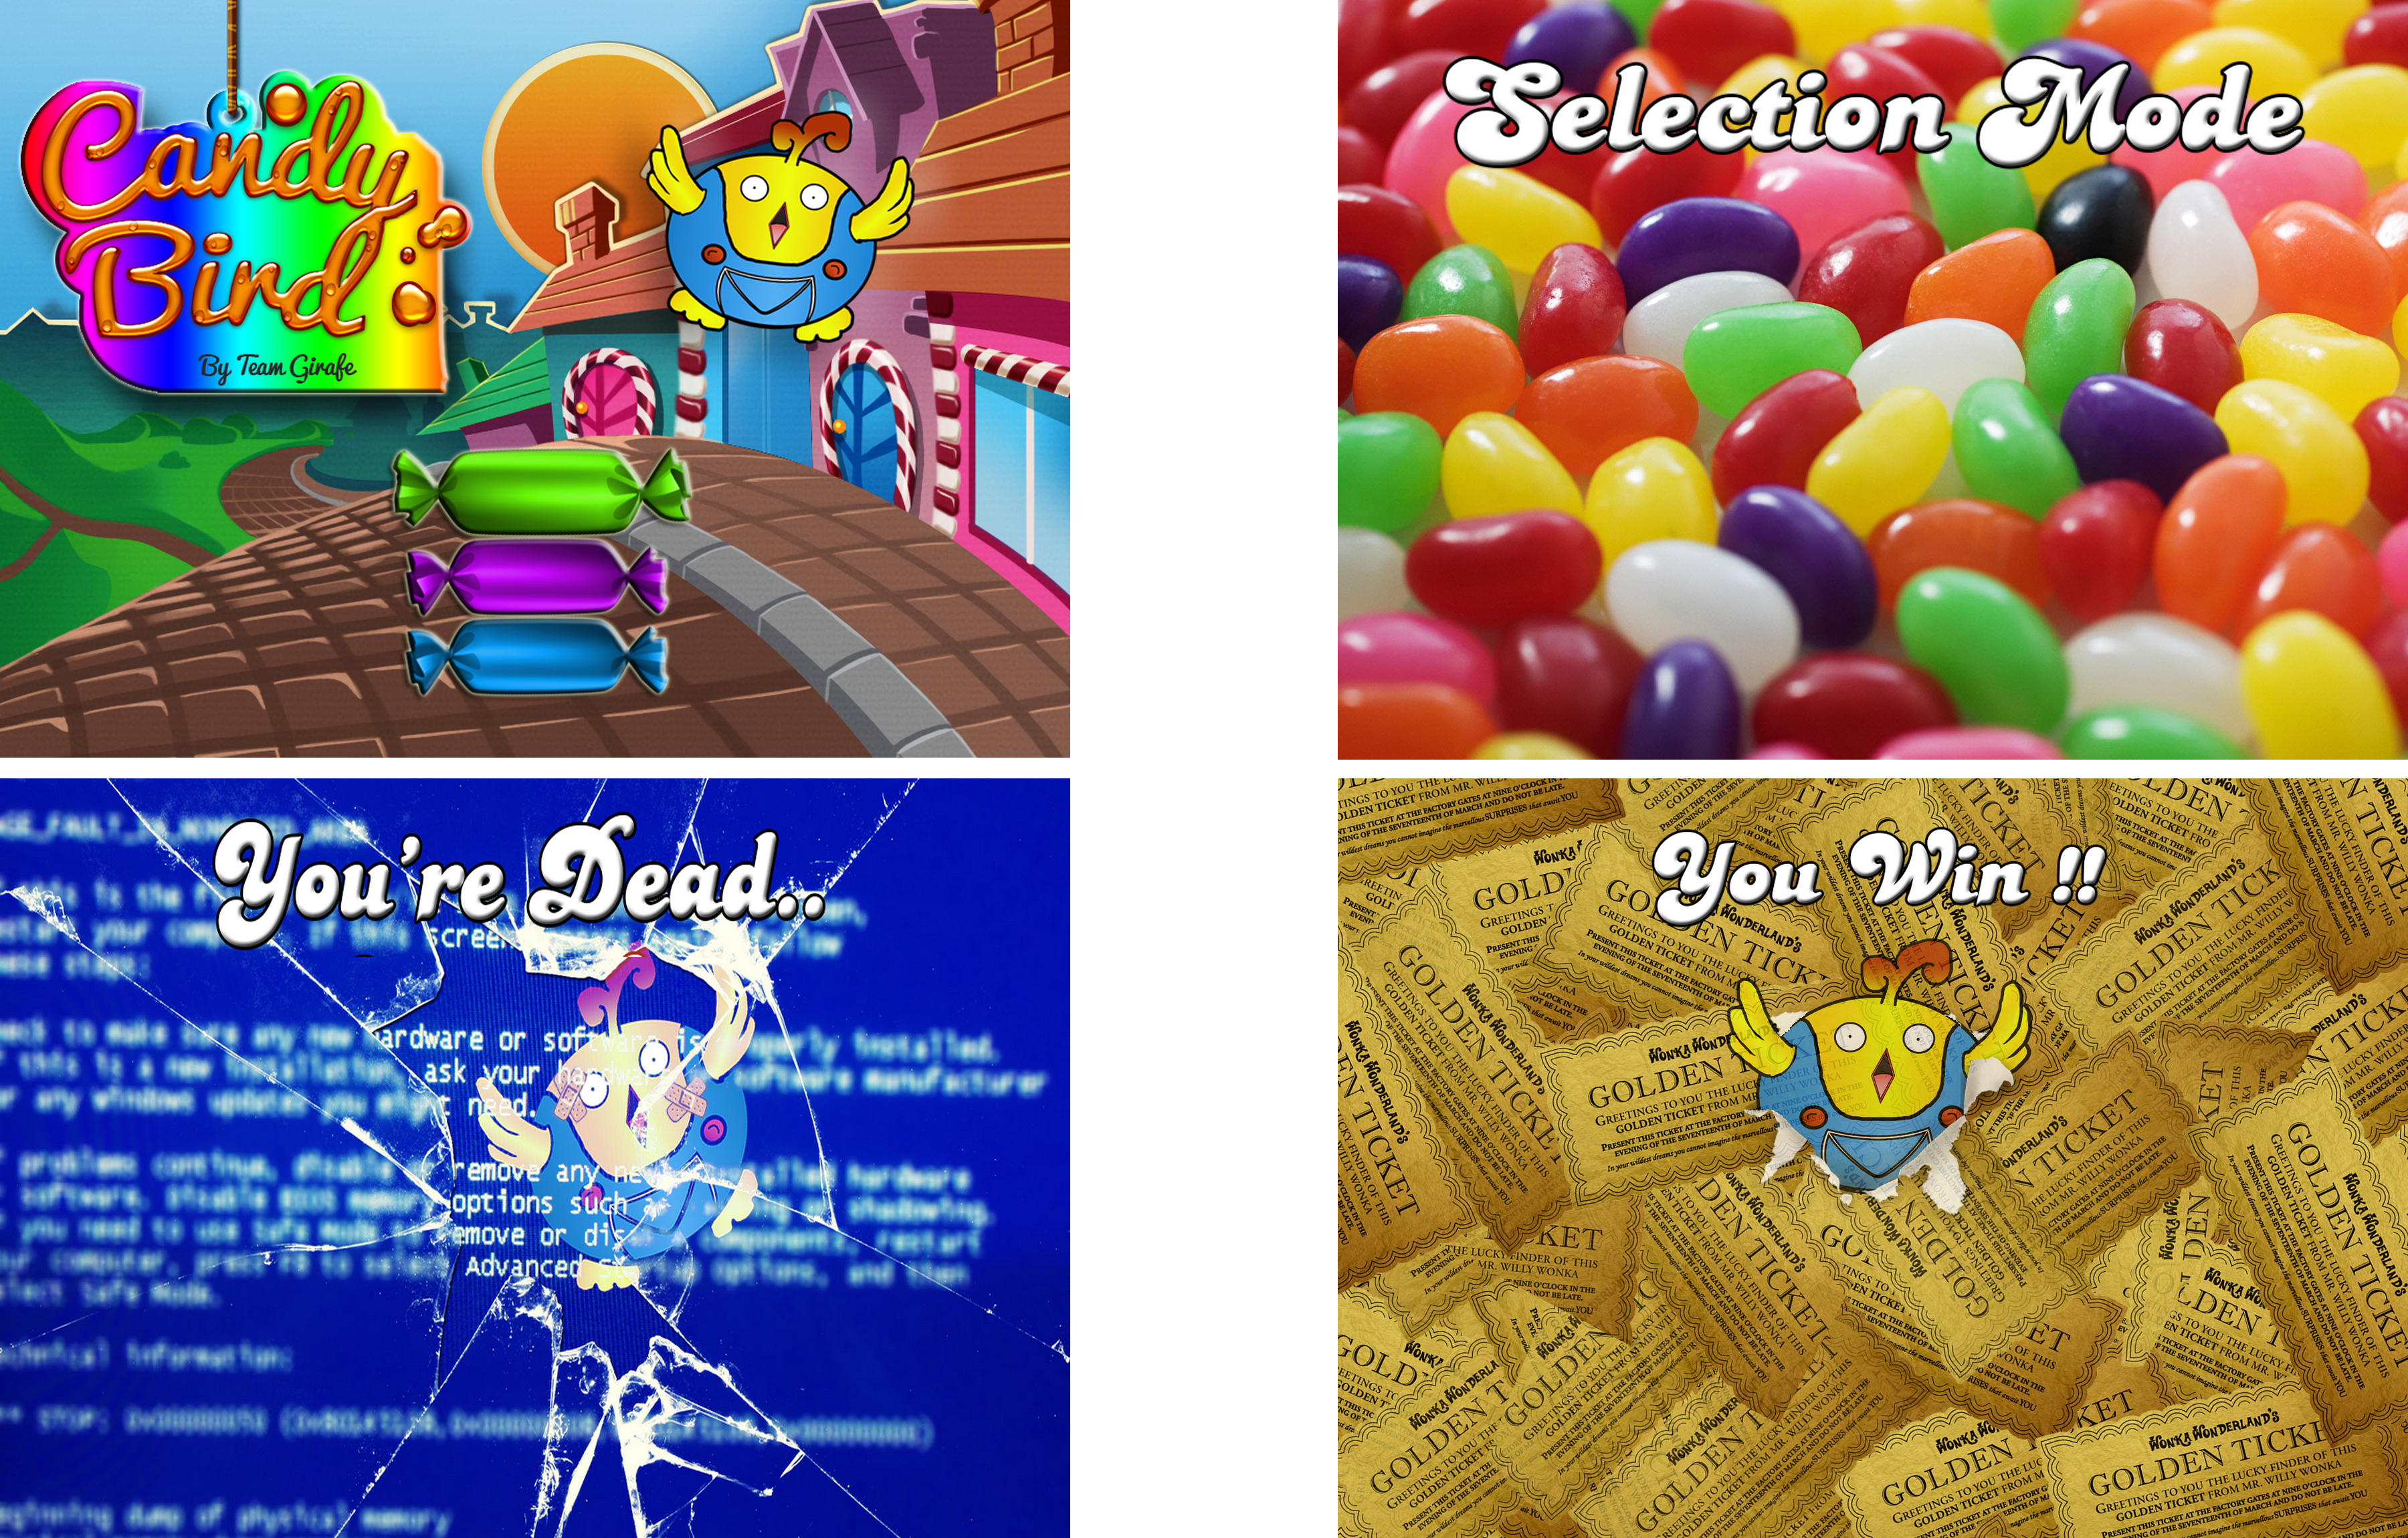
\includegraphics[scale = 0.1]{images/Menus.png}
		\end{center}
		
		
		\vspace{10mm}
			 
			 
		
		Mais bien évidemment il faut des liens entre ces pages pour passer de l'une à l'autre. Dans les premiers jours de code, nous avons rencontré quelques difficultés dans l'agencement de ces états puisque tout était placé dans le Game1 et ce n'était donc vraiment pas simple de s'y retrouver et de modifier correctement les updates nécessaires et des bons affichages. En écoutant des étudiants de niveau supérieur, la solution la plus claire était de faire une pile d'état qui n'afficherait et ne mettrais à jour que le haut de la pile.\\
		
		Après des recherches, quelques tests et des ratés face à cette utilisation de pile, la combinaison d'une énumération d'états et d'un switch s'est avérée correspondre aussi bien à nos attentes. Cela nous a permis de simplifier au maximum le code dans le Game1 et de créer des Classes pour chaque états.\\
				
		\noindent Morceau de code extrait de l'update() actuel du Game1 :
		
		
		\begin{mylisting}
	switch (CurrentGameState)
	{
		case GameState.MainMenu:
			MenuMain.Update(gameTime);
			break;
			
			.
			.
			.
			
		case GameState.Win:
			MenuWin.Update(gameTime);
			break;
	}
				\end{mylisting}
		
		\vspace{10mm}
		
		Avec cette configuration, chaque état a sa propre Classe. Le Game1 se retrouve donc largement simplifié puisqu'avec le switch il sait quel État actualiser ou afficher.\\
		
			
		C'est, comme vous l'aurez sans doute compris, dans le "GameState.Playing" que le gros du jeux va se passer puisque c'est ce qui correspond à une partie (dans un des deux modes).
		
		
		\vspace{10mm}
		\newpage
		
		
		
	\section{\'Editeur de Map}
						
			Nos cartes sont représentées avec différents chiffres correspondant à des blocs. Par exemple, lorsqu'il y a un "0", cela signifie qu'il y a une case de vide à cet emplacement. Le second bloc à retenir est le "1". C'est lui qui représente la ligne d'arrivée (qui une fois franchie nous fait gagner) dans le mode histoire. Le "2" quand à lui va représenter le fameux bonbon que notre oiseau recherche tant et qui lui permettra de gagner à nouveau de l'énergie. Les autres blocs sont les obstacles infranchissables, ils n'y a pour l'instant que deux types d'obstacles. Nous n'utilisons donc que le "3" et le "4".\\
			
			\indent Maintenant que vous avez compris de quoi se compose une map, vous serez d'accord avec nous pour dire que les écrire à la main peut devenir terriblement long et très vite lassant. C'est pour cela que nous avons créé un éditeur de maps qui écrira lui même dans le fichier .lvl de façon à ce que nous ayons juste à cliquer un peu partout pour avoir une jolie map.
			
			\vspace{10mm}
			
	\noindent Screen de la bête : 
						
		\vspace{4mm}
		
			\begin{center}
			\includegraphics[scale = 0.4]{images/EditeurMap.png}
			\end{center}
			
			
			
		\newpage
			
			
			
			Nos Maps sont basées sur des fichiers textes (en .txt) que nous renommons en .lvl pour level (sans blagues). Le fichier est composé de:\\
						
						\indent- une première ligne indiquant le nombre de lignes de blocs où seront placés des \\\indent obstacles ou des bonbon.\\
						
						\indent- une deuxième ligne indiquant cette fois le nombre d'éléments à afficher sur chaque\\\indent ligne. C'est donc l'affichage horizontale du jeu.\\
						
						\indent- un ensemble de ligne de même longueur (que nous mesurerons pour la création de \\\indent la carte) permettant de placer tous les éléments à différents emplacements sur la carte\\\indent selon la ligne ainsi que la colonne sur laquelle ils se positionnent.
						
						
						\vspace{10mm}
						
						\begin{center}
							\includegraphics[scale = 0.6]{images/lvl.png}
						\end{center}
						
						\vspace{10mm}
			
			
		
			 	
			 \indent Lors de la création de l'éditeur de map nous avons eu différents problèmes. Tout d'abord lors de la création des éléments visuels tels que les boutons, n'ayant pas de graphiste dans le groupe, cette tache nous a pris plus de temps que prévu. Au niveau de la création de la partie fonctionnelle de l'éditeur de map, nous ne savions pas du tout comment nous y prendre. Puis, après avoir étudié nos besoins et ceux des utilisateur, nous avons pu mettre en place les différentes parties de notre éditeur. Skeat et Vincae se sont partagé le travail.
			 
			 Vincae s'est occupé de toute la partie affichage des différents obstacles et bonbons afin de faciliter la vision d'ensemble d'un niveaux ainsi que du chargement de map existante et de la sauvegarde des maps.\\
			 
			 
			 
	\newpage
		
	La fonction SaveMap : 
			 
 	\vspace{10mm}
			 
	 \begin{mylisting}
	
      for (int j = 0; j < mapHeight; ++j)
      {
        if(j > 0)
           objWriter.WriteLine("");
        for (int i = 0; i < mapWidth; ++i)
        {
           objWriter.Write(layer[i, j]);
        }
      }
      
	\end{mylisting}
		
		
		\vspace{10mm}
		
		
		
		Dans cette partie du programme qui permet la sauvegarde d'une carte à partir de  notre éditeur, nous utilisons deux boucles imbriquées. La première gère les lignes tandis que la deuxième correspond à une place dans cette ligne (ce qui correspond donc aux colonnes).
		
		De cette manière, on parcourt la map dans sa totalité et pour chaque élément on va écrire dans le fichier .lvl la valeur du bloc lui correspondant contenu dans le tableau layer. 
		
		De plus, à chaque début de ligne, exceptée la première, on retourne à la ligne dans notre fichier pour que ce soit bien un bloc uniforme de ligne et non une unique grande ligne.\\
		
		\vspace{10mm}
		
		
		Tandis que Skeat s'est occupé de la modification en temps réel de la map. Cette partie consiste donc à récupérer le bloc que l'utilisateur sélectionne, et le placer à l'endroit souhaité sur la map. Une petite difficultée s'est posée sur cette partie puisqu'il est question de savoir où le clic a été effectué pour placer le bloc au bon endroit dans la matrice de la map puis l'afficher sous la souris, tous ca de façon optimisée pour ne pas faire ramer l'éditeur.\\
			 
			
	
	
	\newpage
	
	\section{Réseau}
	Comme expliqué dans l'introduction, notre jeu permet, si l'on se connecte au démarrage du jeux, d'envoyer le score à la base de données de notre site web.\\
	
	Avec quelques tutos en ligne et les connaissances de T4ze dans le domaine du Web, la compréhension des fonctions nécessaires fut assez simple et l'implémentation fonctionnelle rapidement.
	
	La gestion de ce qui concerne la base de donnée (lecture, écriture, test) utilise une Dll nommée "Mysql.Data" car il n'est, par défaut, pas possible de faire communiquer un environnement de jeux en C\# avec une base de données en MySql. Cette Dll est disponible en téléchargement libre sur internet et se trouve très simplement; parfois même avec des exemples de fonctions. Mais nous avons préféré tout reprendre nous même pour avoir un code propre, optimisé et surtout que nous contrôlons entièrement.
	
	Pour la comprendre et pouvoir la contrôler sans faire planter notre jeux, nous avions préalablement implémenté la classe DBConnect.cs dans un projet annexe. Nous avons ainsi pu tester les fonctions d'ajout de données, de suppressions, de mises à jour, de tests d'existence de valeur et de listages au fur et à mesure qu'elles étaient écrites. Certaines fonctions créées ne nous sont pas utile dans l'état actuel du jeu. Mais puisque nous étions sur notre lancée et dans une pensée d'améliorations possibles du jeux si nous voulons par la suite, par exemple, rajouter des options telles que s'inscrire depuis le jeux, afficher le classement ou encore changer de pseudo, elles seront déjà prête.\\
	
	\vspace{4mm}
	
	\noindent Forme de la base de donnée avec laquelle le jeux communique :
	\begin{center}
		\includegraphics[scale = 0.8]{images/Bdd.png}
	\end{center}
		
		
	\vspace{10mm}
	
	Comme vous pouvez le voir sur le screen de la base de données, pour plus de sécurité nous chiffrons votre mot de pass en md5. De cette façon, même si un individu parvenait à s'infiltrer dans notre site (quasiment impossible vu notre sécurité), il ne pourrait pas modifier votre score, vous êtes donc bien protégé chez nous. C\# contient une méthode de chiffrement md5 qui nous facilite grandement le test de correspondance de mot de passe puisqu'à notre niveau, implémenter ce chiffrement aurait été vraiment compliqué.
	
		
	\newpage
	
	Toute cette partie nous sert à ceci : Le classement inter-joueur
	
	\begin{center}
		\includegraphics[scale = 0.6]{images/classement.png}
	\end{center}
			
	
	
	\vspace{10mm}

	L'envoi du score se fait uniquement en mode Map Infinie (le score ne se base que sur le nombre de mètres parcourus, il n'y a pas donc pas de score comptabilisé sur les maps prédéfinies). Cet envoi est réalisé en fin de partie, lorsque vous avez perdu et uniquement si vous vous étiez au préalable connecté à votre compte CandyBird. Cet enregistrement est obligatoire car sans lui vous n'existez pas dans la base de donnée et donc votre score n'est pas comptabilisé dans le classement.
	 
	 \newpage
	 
	\section{Site Web}
	
	URL du site web : 
	\begin{Verbatim}
	http://www.CandyBird.eu/
	\end{Verbatim}
	
	Dans un esprit pédagogue, nous avons choisis de réaliser notre site à la main plutôt que d'utiliser un CMS (Wordpress ou autre). T4ze avait déjà, auparavant, monté différents site web et il a ainsi pu s'occuper de cette partie sans trop de problèmes. Le site regroupe actuellement une présentation rapide de notre projet accompagnée d'images qui illustrent les différentes parties de notre jeu. Chaque membre du groupe a sa page personnelle, avec une petite présentation ainsi qu'une photo (la classe). Pour la partie pratique, vous pouvez télécharger nos différents rapports, en LaTeX ou en PDF, ainsi que la version du code source présenté lors des différentes soutenances directement depuis le site. De plus, une page est réservée à l'inscription (avec enregistrement de carte bleu tout ça tout ça... histoire de rembourser tous nos frais de l'année). Cette partie n'est pas obligatoire mais recommandée puisque qu'il faut se connecter au jeux pour accéder au mode multijoueur et avoir l'envoi de score en ligne en fin de partie.\\
	\vspace{4mm}
	
	\begin{center}
	\includegraphics[scale=0.5]{images/site.png}
	\end{center}
	
	\vspace{10mm}
	
	Pour rester à l'écoute de nos admirateurs, une page de contact est disponible. Vous avez donc la possibilité de nous laisser des commentaires ou de nous suggérer des améliorations (pas de signalement de bugs puisque nous codons assez bien pour qu'il n'y en ai pas). Et pour ceux qui aiment être toujours informé, nous tenons une page facebook dont un raccourci est visible sur le site (à gauche dans le pied de page).
	
	\vspace{10mm}
	
	\newpage
	
	\section{Graphique}
	La partie graphique du projet a été compliquée suite au départ imprévu d'Adrien. C'était lui qui était le plus expérimenté face aux logiciels d'édition d'images (Photoshop en l'occurrence). Il a donc fallu  très vite apprendre les bases de ce logiciel afin de pouvoir réutiliser et modifier les travaux qu'avait déjà produit Adrien. Ce petit problème n'était pas des moindre puisqu'un jeu avec des graphismes mal finis n'est pas très agréable à jouer et nous le savons bien.
	
	\indent Nous n'avons pas de personne directement assignée au graphisme, chacun crée les graphismes dont il a besoin au fur et à mesure que nous avançons dans nos parties. Ce n'est pas forcément très efficace mais cela évite qu'un des membres se consacre entièrement au graphisme au détriment du code car ce n'est pas un projet de graphisme. Nous souhaitons que chaque membre puisse apprendre ce qu'il souhaite, c'est pour cela que nous sommes parfois peut-être trop nombreux sur une même tâche, mais cette méthode a l'avantage d'impliquer l'ensemble de l'équipe a 100\% dans le projet.\\*
	\indent Nous avons tout de même défini et suivi un modèle de départ pour partir sur les mêmes bases afin de ne pas se retrouver avec des thèmes décalé d'une partie à l'autre. Chaque modification est montrée à tout les membres de l'équipe pour qu'ils puissent donner leur avis et valider ou non.
	
	\vspace{15mm}
	
	\subsection {Sprite}
	Le personnage principal n'étant pas tellement d'accord avec la façon dont on se sert de lui dans le jeux, bien qu'il ait fermé les yeux sur cette utilisation, il a préféré rester quelque peu dans l'ombre (ce qui explique sont allure étonnemment sombre et ses yeux fermés).
	La planche de sprite que nous utilisons proviens de la source d'un projet qui a été annulé et rendu open source. Nous nous sommes permis de la récupérer et de la modifier à notre convenance.
	
	\vspace{4mm}
		
		\begin{center}
		\includegraphics[scale=0.5]{images/bird.png}
		\end{center}
		
	\vspace{10mm}
		
	Le jeux étant en 2D, seul le profil de l'oiseau nous intéresse. Le personnage est donc géré via un spritesheet, une image qui comporte les détails des mouvement du personnage. Six animations s'enchainent en boucle pour faire bouger ses ailes et ses pattes rendant ainsi son vole plus réaliste.
	

	
	
	
\chapter{Et Après?}
	\section{Map Editor 2.0}
	L'éditeur de map sera intégré au jeu afin que vous puissiez créer vos propres maps et ainsi étendre la durée de vie de notre jeu (qui est déjà infini), vous aurez aussi la possibilité de mettre au défi vos amis en partageant vos créations, ce qui rendra le jeu quelque peu plus addictif.
	
	
		
		\vspace{10mm}
	
	
	
	\section{Réseaux Multijoueur}


	
	\vspace{10mm}



	\section{Nouveaux Personnage}
	Nous savons que notre bel oiseau est très attachant, mais nous avons décidé de rajouter de nouveaux personnages, qui auront des caractéristiques physiques différentes, pour que vous puissiez choisir un personnage qui vous corresponde le mieux possible.
	
	
		
		\vspace{10mm}
	
	
	
	\section{Graphismes}
	
\newpage

\chapter*{Conclusion}
\addcontentsline{toc}{chapter}{Conclusion}

C'est bien stylé.





\end {document}